Wave phenomena occur throughout nature in many forms. As Nikola Tesla puts it: ``If you want to find the secrets of the universe, think in terms of energy, frequency and vibration''. Examples include:
\begin{itemize}
	\item Electromagnetic waves~\cite{Dobbs1985ew} with application into dental radiography (X-rays), microwave ovens, television, radios, just to name a few.
	\item Seismic waves with application including predicting tsunamis~\cite{Bernard2009t} and volcano eruptions~\cite{Brenguier2008tfv}.
	\item Structural vibrations with applications into noise prediction and control, architectural and musical acoustics.
	\item Acoustic waves with applications in ocean acoustics and acoustical oceanography\cite{Munk2009oat,Iorio2017tyo}. 
\end{itemize}
In this thesis the focus is mainly on acoustic waves, but also in combination with structural vibration, namely how sound and structures interact~\cite{Junger1986ssa}. The study of acoustic-structure interaction (ASI) is the topic of the first two papers while the latter two are restricted to the fluid part. Acoustic waves are used to detect and localize objects~\cite{Lurton2002ait}, for underwater communication, and for remote sensing of the ocean: to remotely classify distributions of biological organisms such as fish~\cite{MacLennan1989amo} and plankton~\cite{Stanton2000rar}, for the purpose of fish supply management and ecological studies~\cite{Pena2008mtt}; to characterize the seafloor micro relief, with application in sound propagation, geological studies and mining; to remotely measure physical properties of the ocean such as temperature, flow and turbulence, with applications in climate monitoring~\cite{Consortium1998occ} and the study of bottom boundary layer dynamics and hydrocarbon seeps. 

Common for all applications above is the possibility to linearize the governing equations such that the problems may be modeled by the much simpler wave equation
\begin{equation}\label{Eq:waveEquation}
	\nabla^2 \breve{p} = \frac{1}{c_{\mathrm{f}}^2}\pderiv[2]{\breve{p}}{t}
\end{equation}
with wave speed $c_{\mathrm{f}}$. Looking for solutions of the form $\breve{p}(\vec{x},t)=\euler^{-\imag\omega t}p(\vec{x})$ (with angular frequency $\omega$) the wave equation may be analyzed in the frequency domain as the Helmholtz equation
\begin{equation}
	\nabla^2 p + k^2 p = 0
\end{equation}
with the wave number $k=\omega/c_{\mathrm{f}}$. 

\Cref{Fig:physicalProblem} illustrates the general problem setup considered in this thesis. For subsurface acoustics, the unbounded domain $\Omega^+$ is modeled as water whereas internal fluid domains may either be water or air (i.e. pressure hulls in submarines). Sound signals is the only practical way of transmitting sound in water~\cite{Jensen2011coa}, and so an understanding of the physical properties of such signals are important, not only for sonar (sound navigation ranging) technologies, but also the study of marine life. The precise behavior of subsurface sound waves is dependent on a vast set of parameters including the temperature, the salinity and the depth. In this work, however, linearized equations like the wave equation in~\Cref{Eq:waveEquation} will be used with constant sound speed, $c_{\mathrm{f}}$. That is, the fluid domains are assumed to be homogeneous.
\begin{figure}
	\centering
	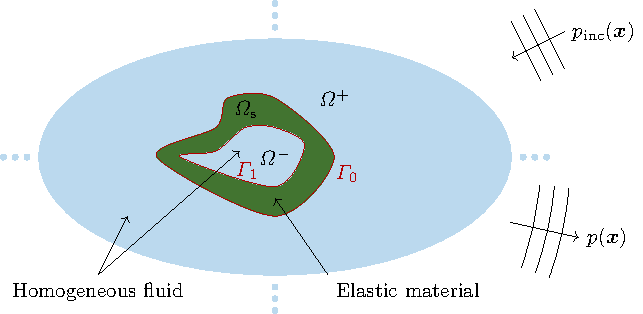
\includegraphics[scale=1]{../../LaTeX/createFigures/TikzFigures/articleIGA_PhD/physicalProblem}
%	\includegraphics[scale=1]{\graphicsFolder/Figure1}
	\caption{Illustration of the physical problem. A plane incident wave, $p_{\mathrm{inc}}(\vec{x})$, is scattered by the scatterer, $\Omega_{\mathrm{s}}$, in an unbounded domain, $\Omega^+$, resulting in the scattered wave, $p(\vec{x})$. The scatterer, which is bounded by the boundaries $\Gamma_1$ and $\Gamma_2$, envelops a fluid domain, $\Omega^-$.}
	\label{Fig:physicalProblem}
\end{figure}

Solution of the time dependent wave equation in~\Cref{Eq:waveEquation} may be found by transforming solutions of the Helmholtz equation for a range of frequencies ${f=\omega/(2\PI)}$ using an inverse Fourier transformation~\cite{Jensen2011coa}. This approach is advantageous for several reasons. First, the dimension of the problem is reduced by one, enabling trivial parallelization over the frequencies. Second, the Fourier transformations step may be computed by a fast Fourier transform with a reduced complexity from $\bigoh(N^2)$ to $\bigoh(N\log N)$ with $N$ being the data size. Third, working with elliptic equations is often easier than hyperbolic equations, especially for exterior Helmholtz problems. Finally, many acoustic applications are of narrow-band nature~\cite{Jensen2011coa} leading to a reduction of the spectrum of frequencies in which solutions of the Helmholtz equation are needed.

In three dimensions the scattering problem in~\Cref{Fig:physicalProblem} only admits analytic solutions on closed form for very simple geometries. The scarcity of such solutions makes the existing solution very valuable and is the subject of the first paper. 

For slightly more complex geometries, however, numerical methods are required. To this end, a vast set of methods are available. Finite element analysis is the subject of the second paper, the boundary element method is the subject of the third paper and Kirchhoff approximation is the subject of the fourth paper. Additionally, the ray/beam tracing method is investigated in the appendices. Most of these methods fits very well in the isogeometric framework which will be introduced more thoroughly in the introduction part. Finally, the finite difference method (FDM) should be mentioned as an alternative~\cite{Wang1996fdt}. The FDM is not very suited for the present 3D problem setup (in the frequency domain) due to tedious handling of general geometries. However, it is commonly used for discretizing the time dimension when solving the time-dependent wave equation in~\Cref{Eq:waveEquation} (where the spatial dimensions are discretized with finite elements).

The main application studied in this thesis is acoustic scattering on submarines. In this regards the quantity of interest is the \textit{target strength} defined by
\begin{equation}\label{Eq:TS}
	\TS = 20\log_{10}\left(\frac{|p_0(\hat{\vec{x}})|}{|P_{\mathrm{inc}}|}\right)
\end{equation}
where $P_{\mathrm{inc}}$ is the amplitude of the incident wave at the geometric center of the scatterer (i.e. the origin) and the far field pattern of the scattered pressure, $p$, is given by
\begin{equation}\label{Eq:farfield}
	p_0(\hat{\vec{x}}) =  \lim_{r\to\infty} r \euler^{-\imag k r}p(r\hat{\vec{x}}),
\end{equation}
with $r = |\vec{x}|$ and $\hat{\vec{x}} = \vec{x}/|\vec{x}|$ being the far field observation point. The observation point can be represented in terms of the aspect angle $\alpha$ and elevation angle $\beta$ (see~\Cref{Fig:elevationAspect})
\begin{figure}
	\centering
	\begin{subfigure}[t]{0.49\textwidth}
		\centering
		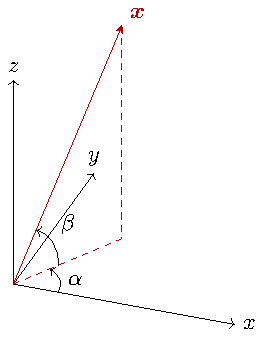
\includegraphics{../../LaTeX/createFigures/TikzFigures/phd/elevationAspect}
	\end{subfigure}%
	\hspace*{0.02\textwidth}%
	\begin{subfigure}[t]{0.49\textwidth}
		\centering
		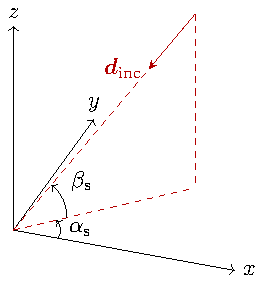
\includegraphics{../../LaTeX/createFigures/TikzFigures/phd/elevationAspect_2}
	\end{subfigure}
	\caption{Illustration of the aspect angle $\alpha$ and the elevation angle $\beta$ describing an observation point $\vec{x}$. The direction of the incident wave can be represented in terms of the aspect angle $\alpha_{\mathrm{s}}$ and the elevation angle $\beta_{\mathrm{s}}$.}
	\label{Fig:elevationAspect}
\end{figure}
\begin{equation*}
	\hat{\vec{x}} = \begin{bmatrix}
		\cos\beta\cos\alpha\\
		\cos\beta\sin\alpha\\
		\sin\beta
	\end{bmatrix}.
\end{equation*}
TS models are also used to discriminate man-made objects, such as mines, toxic waste containers, from natural objects such as rocks. The method known as acoustic resonance scattering utilizes the differences of target strength at low frequencies of natural irregular objects and man-made regular elastic objects~\cite{Zampolli2007bsf,Zampolli2012ltm}. 
\newpage
\section{Background}
The target strength of a submarine is considered highly classified and are typically kept within each nation. The desire to simulate scattering on classified submarines has led to the need of benchmarks not subject to military classification that can be shared such that results could be compared between institutes.

The BeTSSi\footnote{Benchmark Target Strength Simulation.} community gives a solid basis for the benchmarking exercise which is very important for code development. The first BeTSSi workshop was initiated by FWG\footnote{Die Forschungsanstalt der Bundeswehr f\"{u}r Wasserschall und Geophysik. Integrated with WTD 71 (Wehrtechnische Dienststelle f\"{u}r Schiffe und Marinewaffen, Maritime Technologie und Forschung) in 2009.} in 2001 where several models (some of which are illustrated in \Cref{Fig:BeTSSiModels}) were presented as benchmark problems to be analyzed. The first and second workshop were held in Kiel in 2002 and 2012, respectively. The third was held in the Hague in 2016. 

The objective is to compute the target strength of submarine structures. More specifically the analysis of the scattered pressure from a plane wave
\begin{equation}\label{Eq:p_inc}
	p_{\mathrm{inc}}(\vec{x}) = P_{\mathrm{inc}}\euler^{\imag k\vec{d}_{\mathrm{inc}}\cdot\vec{x}}
\end{equation}
incident on the models. Here, $\vec{d}_{\mathrm{inc}}$ is the traveling directing of the plane wave which can be represented in terms of the aspect angle $\alpha_{\mathrm{s}}$ and elevation angle $\beta_{\mathrm{s}}$ (see~\Cref{Fig:elevationAspect})
\begin{equation*}
	\vec{d}_{\mathrm{inc}} = -\begin{bmatrix}
		\cos\beta_{\mathrm{s}}\cos\alpha_{\mathrm{s}}\\
		\cos\beta_{\mathrm{s}}\sin\alpha_{\mathrm{s}}\\
		\sin\beta_{\mathrm{s}}
	\end{bmatrix}.
\end{equation*}
Results from the BeTSSi workshops appears in several publications e.g.~\cite{Schneider2003asb,Nolte2015nmi,Burgschweiger2014rot,Fillinger2014aen,Nijhof2017bis}.
An example of a test case that was presented on the workshop in the Hague was a monostatic\footnote{For \textit{monostatic} scattering we have $\alpha_{\mathrm{s}}=\alpha$ and $\beta_{\mathrm{s}}=\beta$ as opposed to \textit{bistatic} scattering where both the aspect angle and elevation angle in general do not coincide.} sweep over the elevation angles $\beta\in[-\ang{30},\ang{60}]$ at $\alpha=\ang{90}$ of the full BeTSSi submarine (illustrated in \Cref{Fig:FullBeTSSi}) at given frequencies, $f\in[1,3,10,30]\,\si{kHz}$. The institutes that contributed to this benchmark were the DRDC (Defence Research and Development Canada), LR (Lloyd's Register), RAFAEL (Rafael Advanced Defense Systems, Israeli defense technology company), Tel Aviv University, Thales Group, TKMS (ThyssenKrupp Marine Systems), TNO (the Netherlands Organisation for applied scientific research) and WTD 71.
\begin{figure}
	\centering
	\begin{subfigure}{\textwidth}
		\centering
		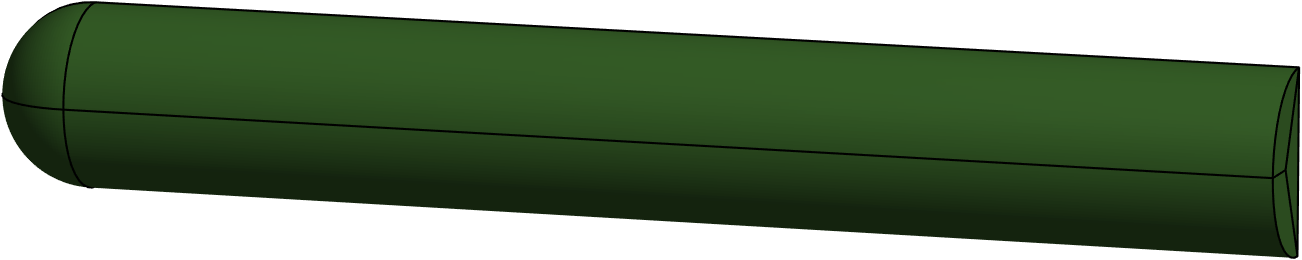
\includegraphics[width=0.6\textwidth]{../../graphics/M1} % width = 0.6613/0.7
		\caption{The BeTSSi model 1 - air filled}
	\end{subfigure}%
	\par\bigskip
	\par\bigskip
	\begin{subfigure}{\textwidth}
		\centering
		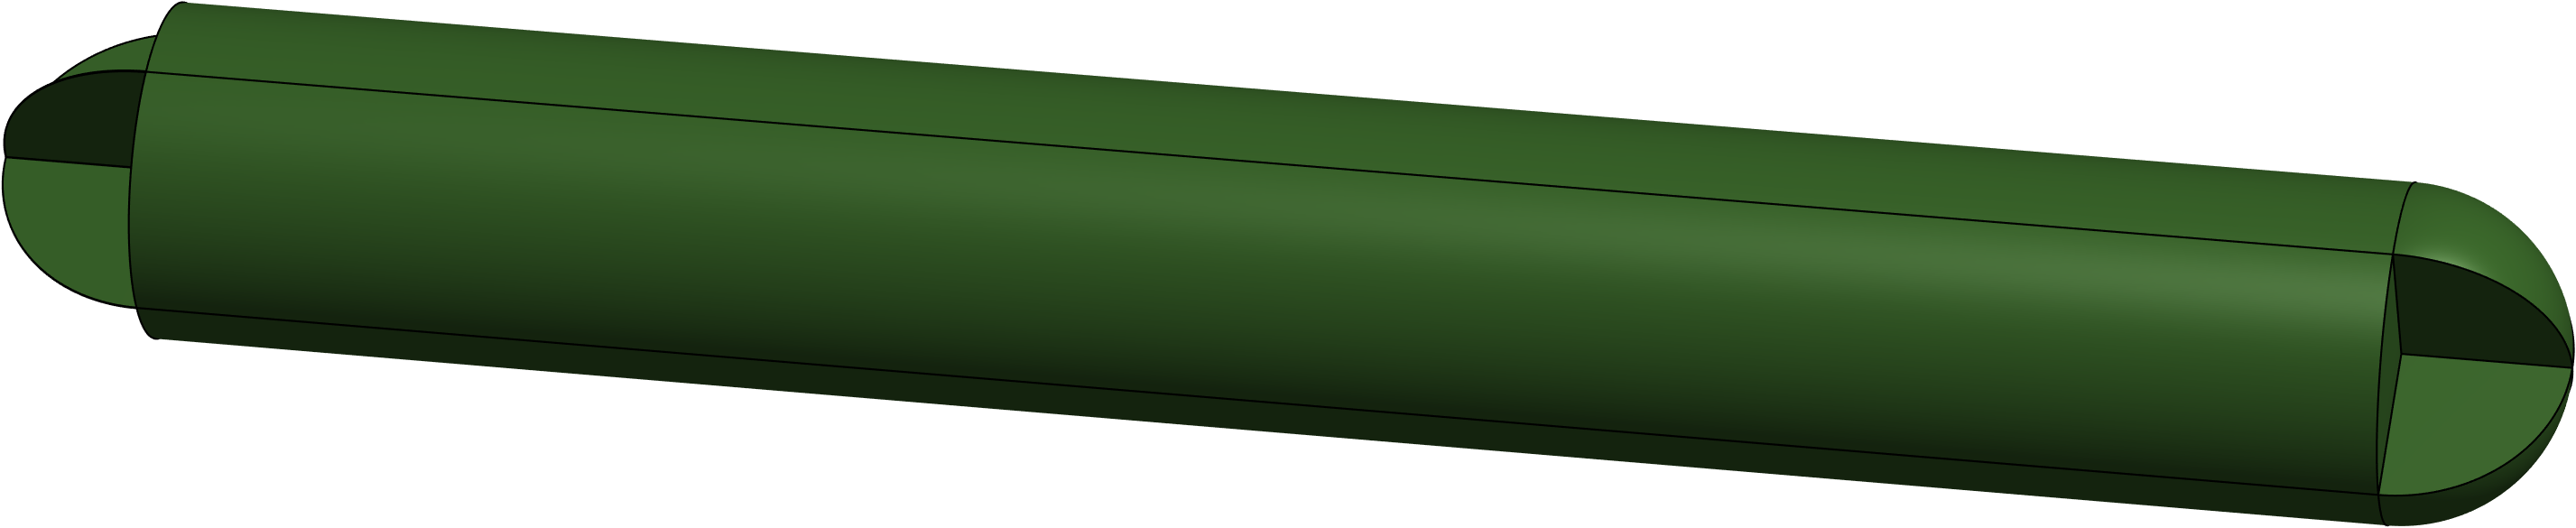
\includegraphics[width=0.6419\textwidth]{../../graphics/M2} % width = 0.6613/0.7
		\caption{The BeTSSi model 2 - air filled}
	\end{subfigure}%
	\par\bigskip
	\par\bigskip
	\begin{subfigure}{\textwidth}
		\centering
		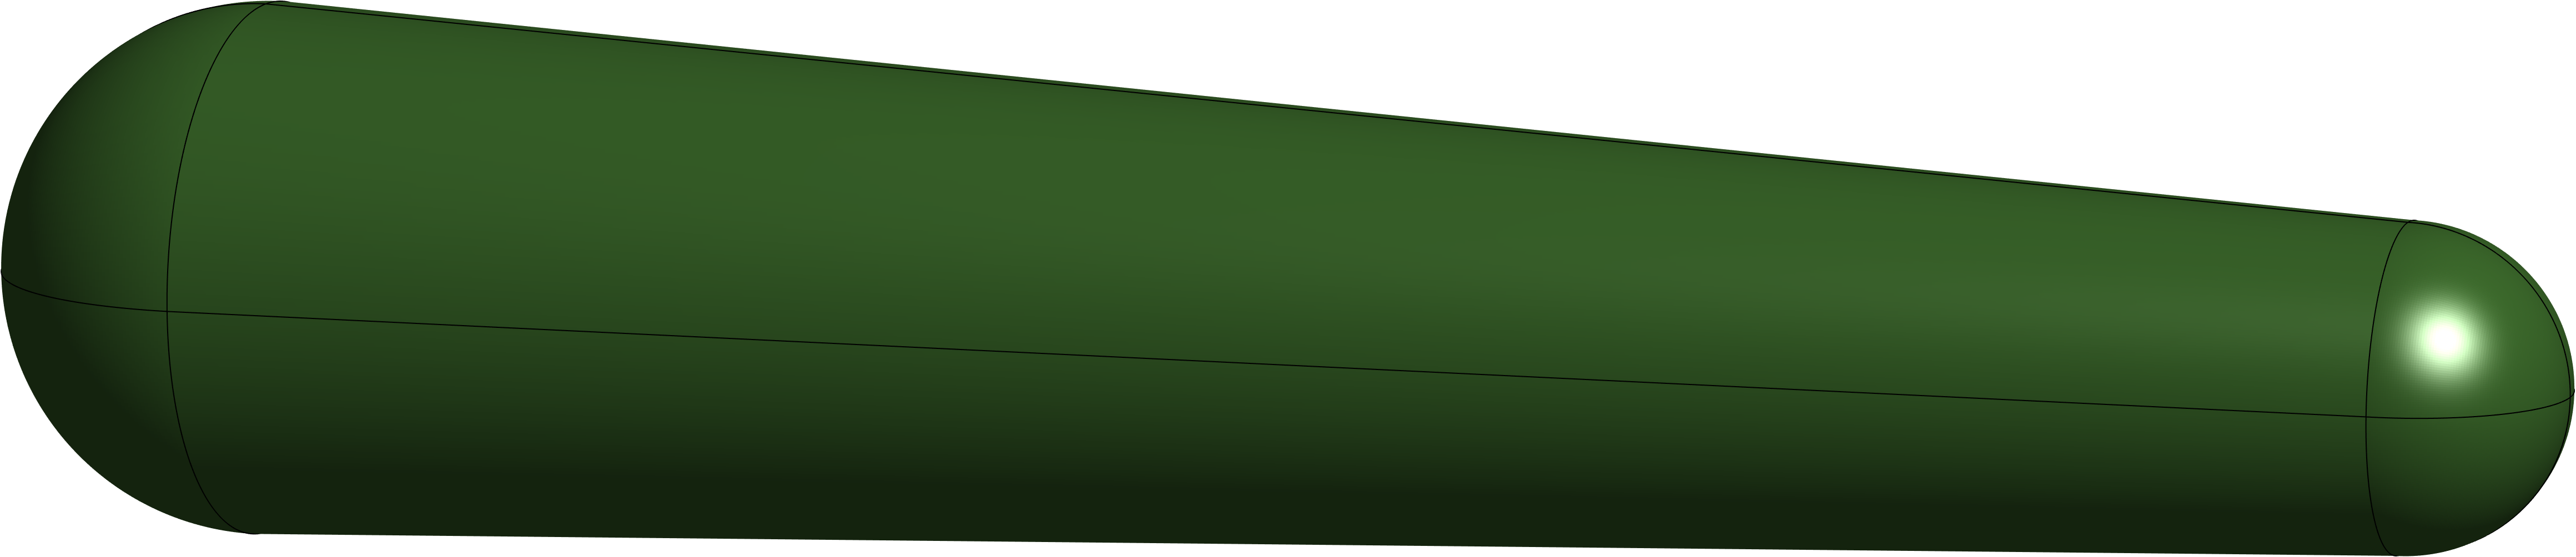
\includegraphics[width=0.76\textwidth]{../../graphics/M3/M3} % width = 0.6613/0.7
		\caption{The BeTSSi model 3 - water filled}
		\label{Fig:BeTSSi_M3}
	\end{subfigure}%
	\par\bigskip
	\par\bigskip
	\begin{subfigure}{0.33\textwidth}
		\centering
		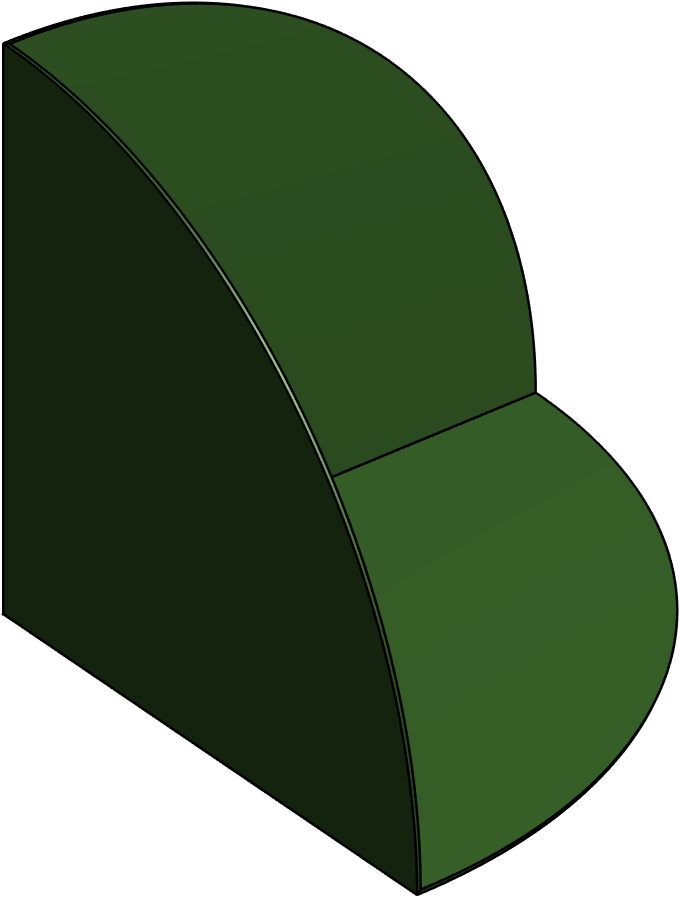
\includegraphics[width=0.3\textwidth]{../../graphics/BeTSSi_M4} % width = 0.6613/0.7
		\caption{The BeTSSi model 4}
	\end{subfigure}%
	\hspace*{0.005\textwidth}%
	\begin{subfigure}{0.33\textwidth}
		\centering
		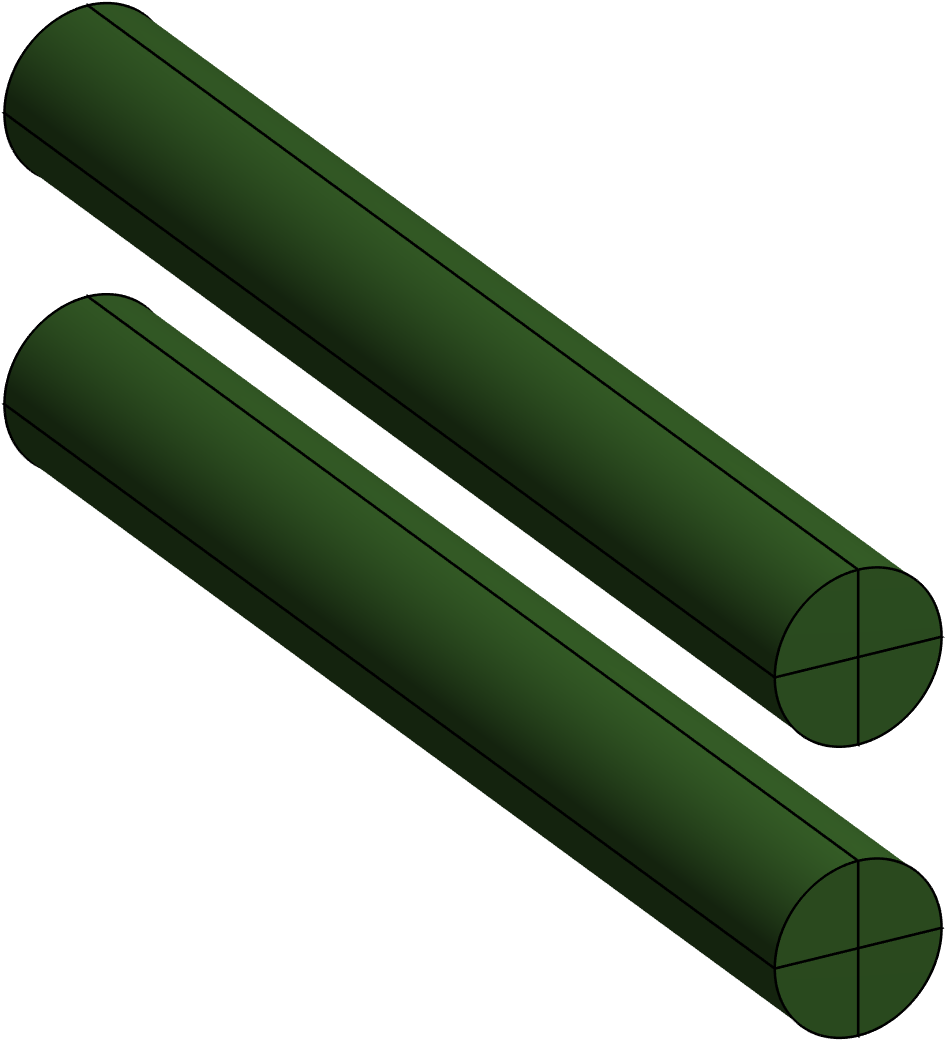
\includegraphics[width=0.45\textwidth]{../../graphics/BeTSSi_M5A}
		\caption{The BeTSSi model 5A}
	\end{subfigure}%
	\hspace*{0.005\textwidth}%
	\begin{subfigure}{0.33\textwidth}
		\centering
		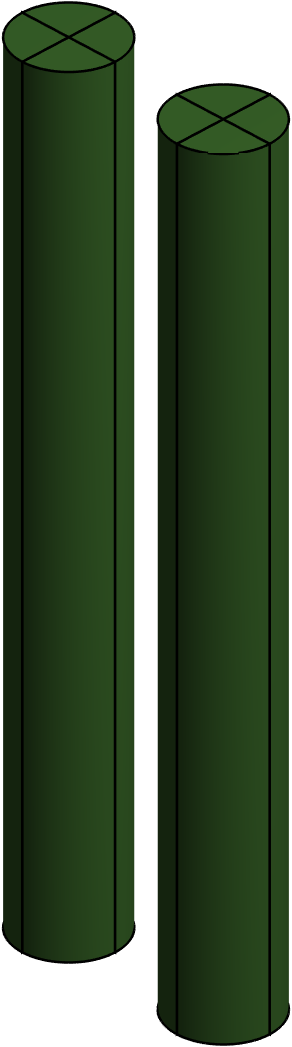
\includegraphics[width=0.2\textwidth]{../../graphics/BeTSSi_M5B}
		\caption{The BeTSSi model 5B}
	\end{subfigure}
	\par\bigskip
	\par\bigskip
	\begin{subfigure}{\textwidth}
		\centering
		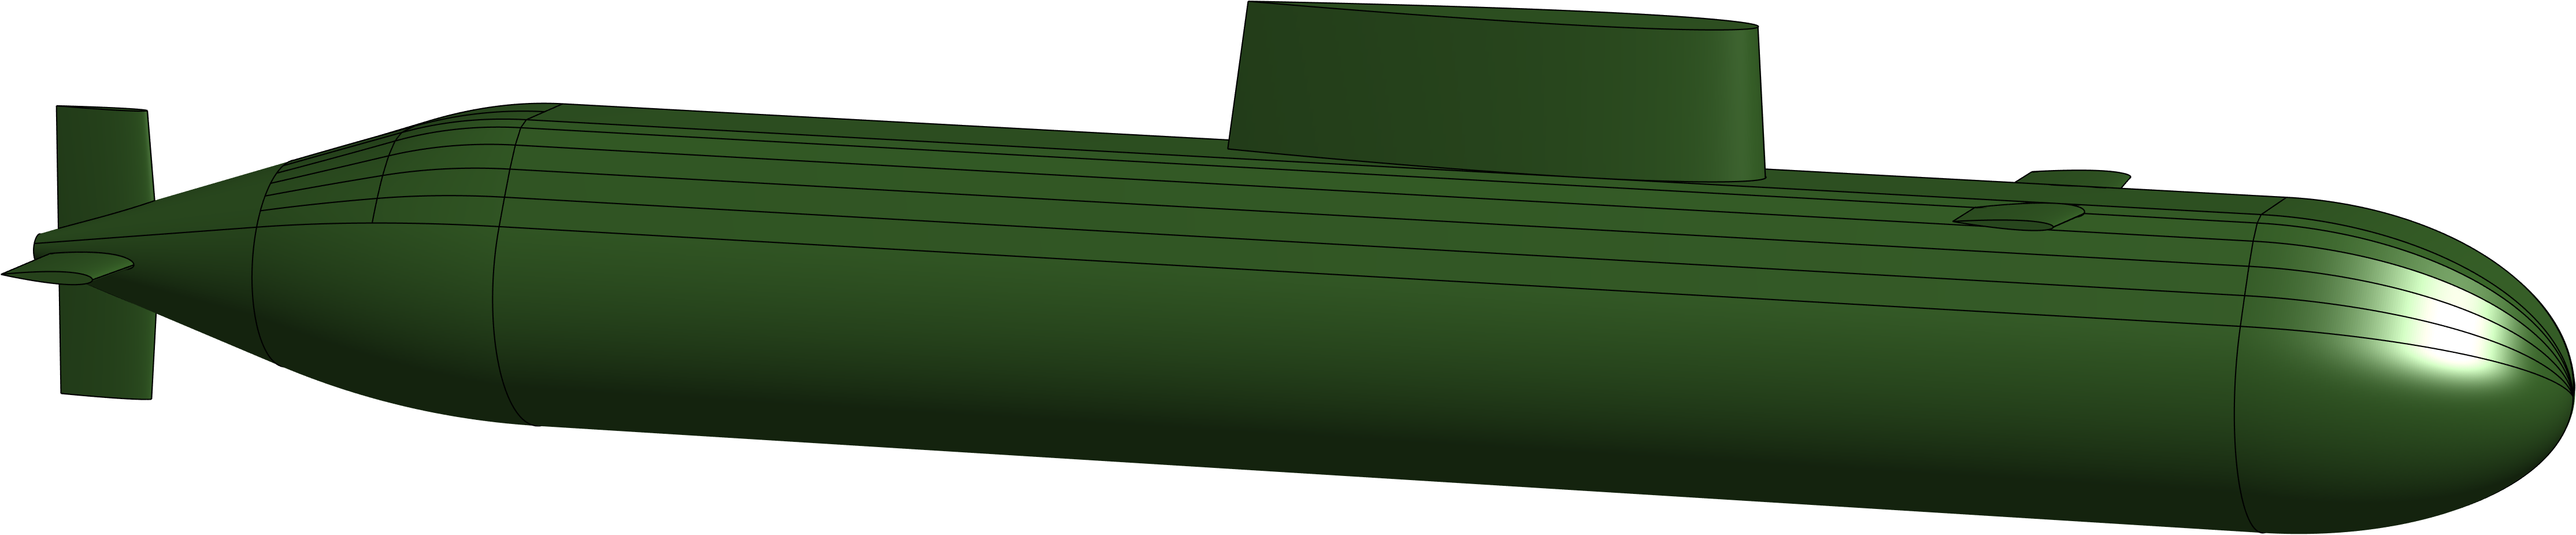
\includegraphics[width=\textwidth]{../../graphics/BCA/CAD}
		\caption{The outer hull of the BeTSSi submarine}
	\end{subfigure}
	\caption{\textbf{BeTSSi models}: The BeTSSi model 3 is described and analyzed in~\cite{Venas2015iao} and the BeTSSi submarine is described and analyzed in~\cite{Venas2019ibe}.}
	\label{Fig:BeTSSiModels}
\end{figure}
\begin{figure}
	\centering
	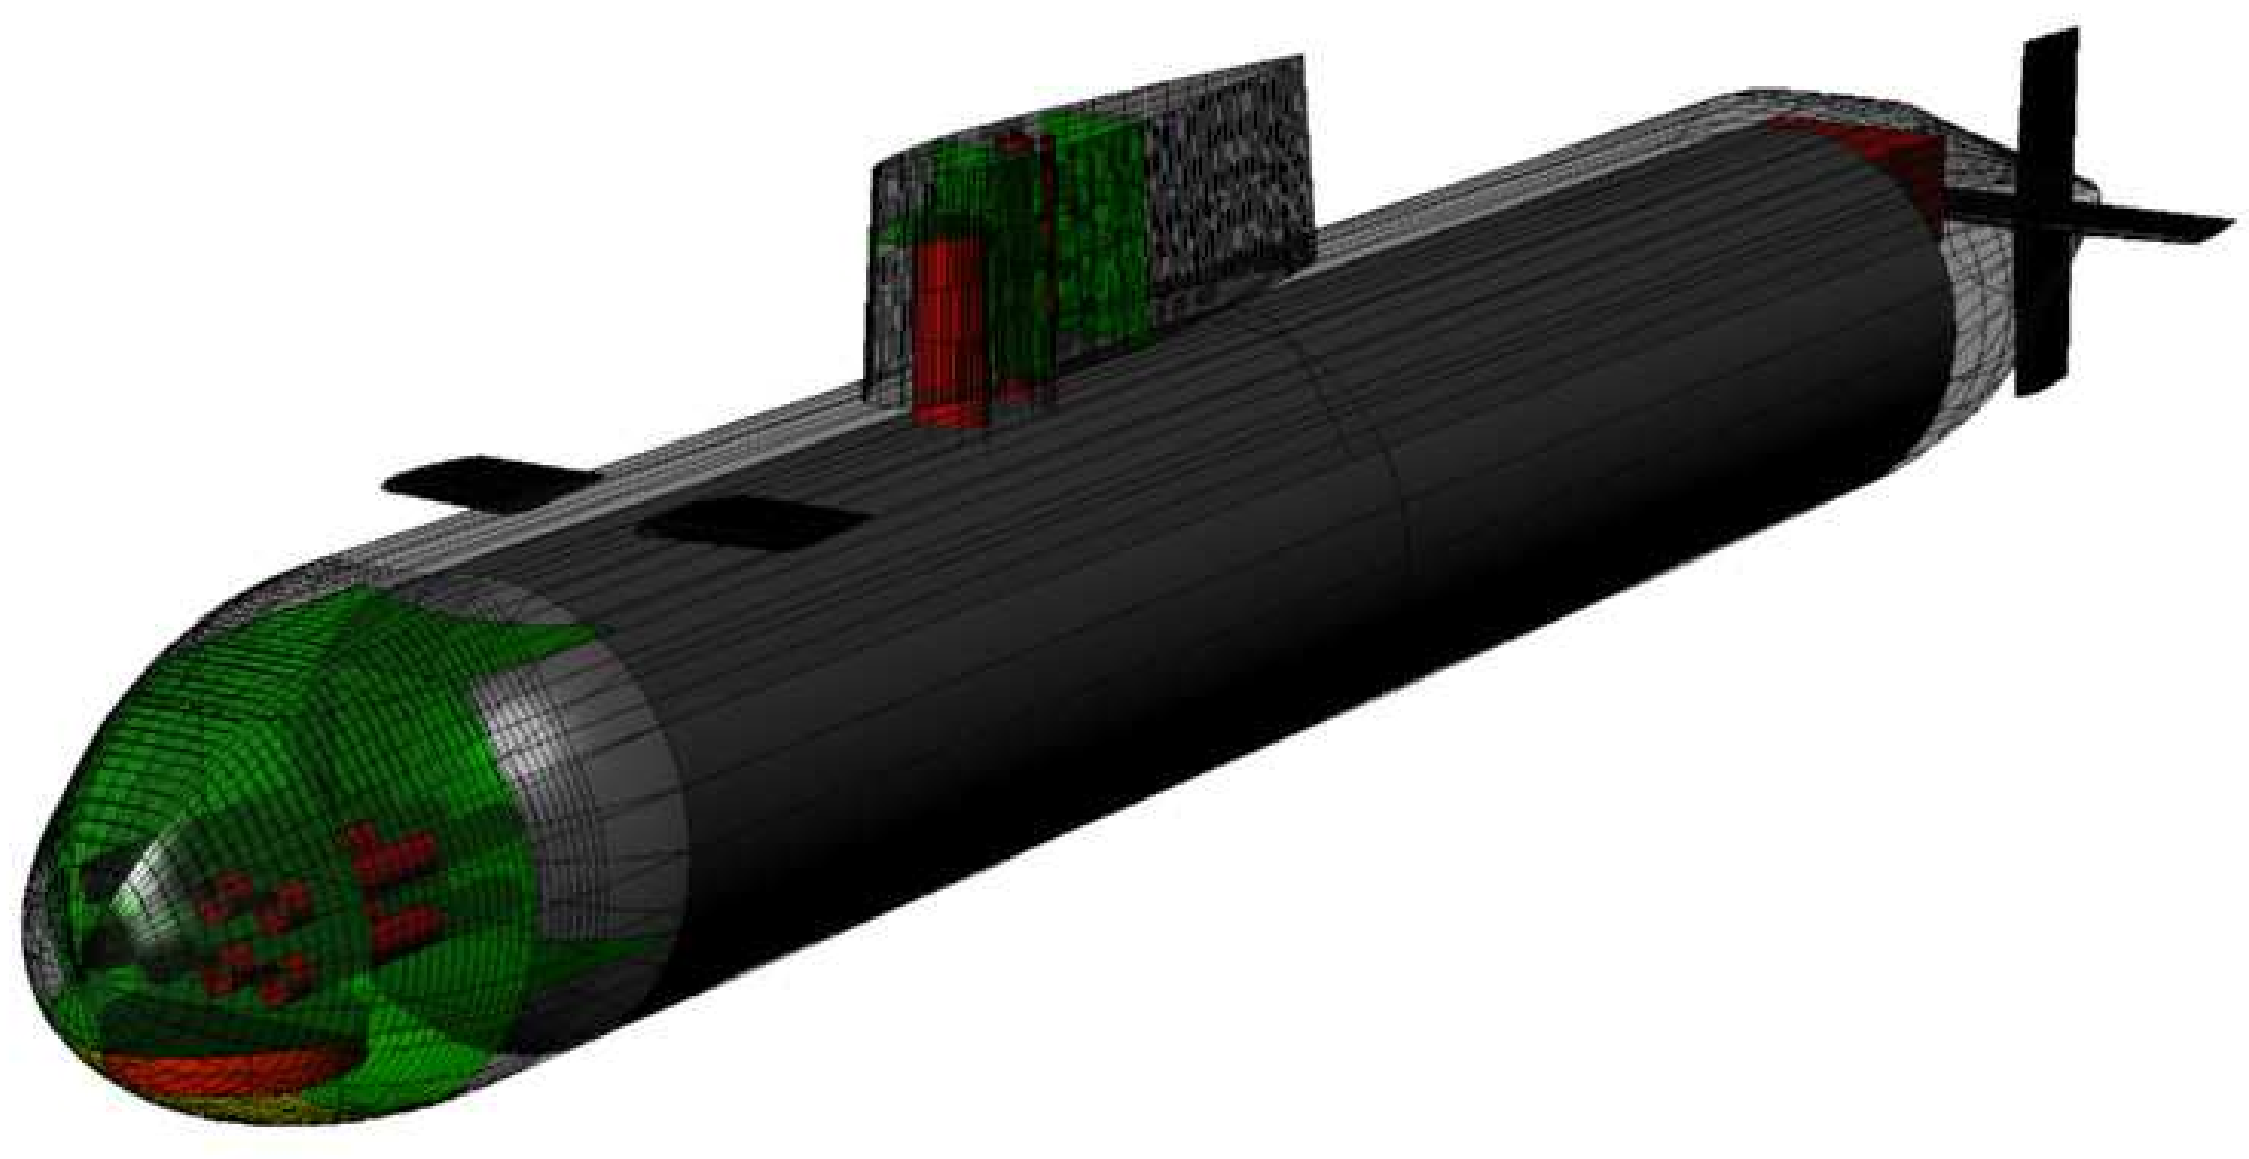
\includegraphics[width=\textwidth]{../../graphics/betssi}
	\caption{The full BeTSSi submarine has internal structures including 8 torpedo tubes, cylindrical hydrophone array, and bulkheads.}
	\label{Fig:FullBeTSSi}
\end{figure}

The results are illustrated in~\Cref{Fig:BT_RBC_MS}. Clearly such a complex benchmark requires advanced software to obtain accurate solutions which are arguably lacking in this benchmark test case. The state-of-the-art is not satisfactory, which is a motivation for the research in the BeTSSi community. To first obtain accurate solutions for simpler benchmark examples is crucial in order to advance to this level of complexity.
\begin{figure}
	\centering
	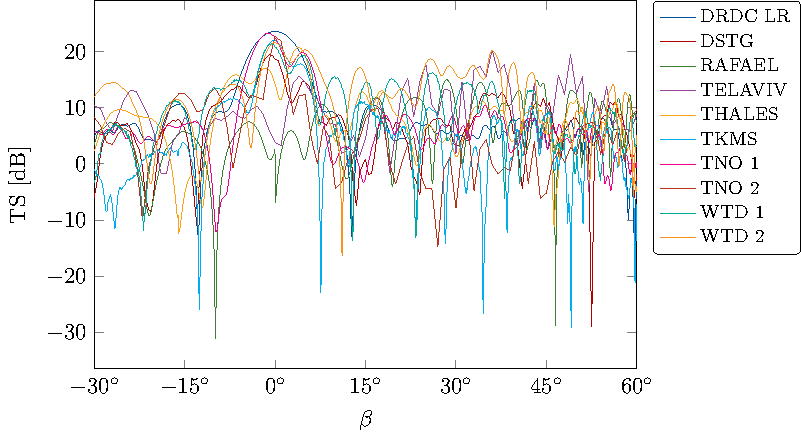
\includegraphics[width=\textwidth]{../../LaTeX/createFigures/TikzFigures/phd/BT_RBC_MS}
	\caption{Monostatic scattering of the full BeTSSi submarine at $f=\SI{1}{kHz}$ sweeping through the elevation angle $\beta$ at $\alpha=\ang{90}$.}
	\label{Fig:BT_RBC_MS}
\end{figure}
It is recommended by the community that the participants first obtain good results on spherical shells which admits analytic solutions~\cite{Venas2019e3s}, before advancing to the BeTSSi models which does not have exact reference solutions available.
A benchmark that will be used throughout this thesis is a plane wave incident in the positive $z$-axis
\begin{equation*}
	p_{\mathrm{inc}}(\vec{x}) = P_{\mathrm{inc}}\euler^{\imag k x_3}
\end{equation*} 
scattering by a rigid unit sphere ($R_0=\SI{1}{m}$). The analytic solution is given by\footnote{Where $\besselj_n(x)$ is the $n^{\mathrm{th}}$ spherical Bessel function of the first kind and $\hankel_n(x)$ is the $n^{\mathrm{th}}$ spherical Hankel function of the first kind.} (expressed in spherical coordinates)
\begin{equation}\label{Eq:S1rigid}
	p(r,\theta) = -P_{\mathrm{inc}}\sum_{n=0}^\infty \imag^n (2n+1) \frac{\besselj_n'(kR_0)}{\hankel_n'(kR_0)} \legendre_n(\cos\theta)\hankel_n(kr)
\end{equation}
Due to axis symmetry, this solution can be generalized for arbitrary incident wave direction (\Cref{Eq:p_inc}) with a simple orthogonal transformation. The advantage of having several models with different complexity is to have a gradual increase in complexity to be able to run simulations on the full BeTSSi submarine. In particular, the BeTSSi model 1 represent a convex model, model 4 represents a triple reflector (which can be found in the more advance BeTSSi model 2) and model 5 represent disjoint geometries. The natural start would be to consider rigid scattering (with hard walled boundary condition) such that only fluid domains need to be modeled. Next, more realistic boundary conditions can be considered which incorporates interaction with elastic shells. The BeTSSi model 1 or 2 may then be embedded in BeTSSi model 3 to check the ability to simulate internal structures. This approach sets the stage for simulating on the full BeTSSi submarine.